\documentclass{xStandalone}

\begin{document}
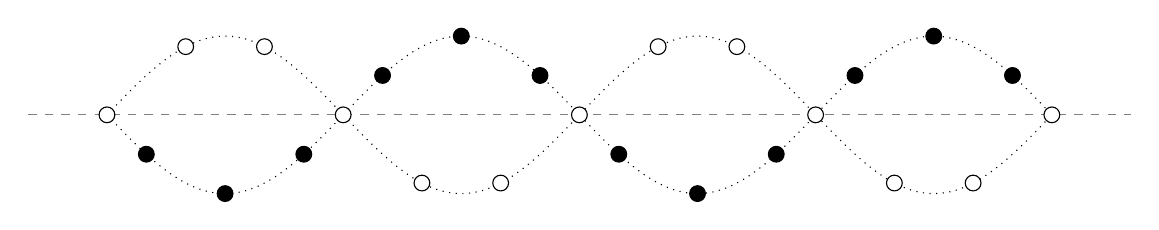
\begin{tikzpicture}

\draw[dashed,gray] (-1,0)--(13,0);

\draw[black,dotted] plot[domain=0:12,samples=1000] (\x,{-sin(deg(\x*2*pi/6))});

\draw[dotted] plot[domain=0:12,samples=1000] (\x,{+sin(deg(\x*2*pi/6))});

\foreach \x in {0,1,...,12}
{
    \draw[fill=white] (\x,\fpeval{+sin(\x*2*pi/6)}) circle (0.1);
}

\foreach \x in {0.5,1.5,...,11.5}
{
    \draw[fill=black] (\x,\fpeval{-sin(\x*2*pi/6)}) circle (0.1);
}


\end{tikzpicture}
\end{document}